% Copyright (c) 2020 Carl Martin Ludvig Sinander.

% This program is free software: you can redistribute it and/or modify
% it under the terms of the GNU General Public License as published by
% the Free Software Foundation, either version 3 of the License, or
% (at your option) any later version.

% This program is distributed in the hope that it will be useful,
% but WITHOUT ANY WARRANTY; without even the implied warranty of
% MERCHANTABILITY or FITNESS FOR A PARTICULAR PURPOSE. See the
% GNU General Public License for more details.

% You should have received a copy of the GNU General Public License
% along with this program. If not, see <https://www.gnu.org/licenses/>.

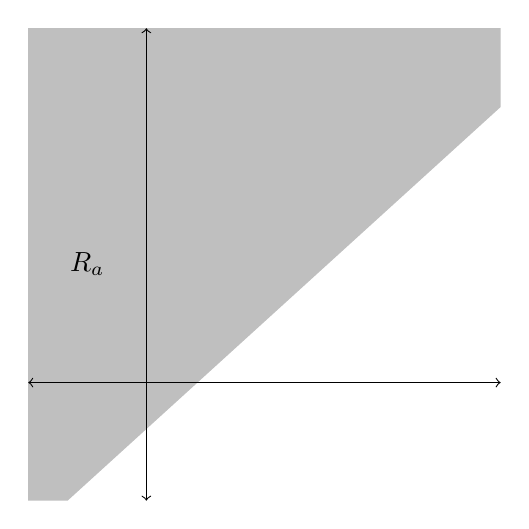
\begin{tikzpicture}[scale=1]
	
	% S'
	\fill[lightgray] (-1,-1.5) -- (4.5,3.5) -- (4.5,4.5) -- (-1.5,4.5) -- (-1.5,-1.5) -- (-1,-1.5);
	\draw (-0.75,1.5) node {$R_a$};

	% % points
	% \fill (0.75,2) circle[radius=1.5pt];
	% \fill (2.75,2) circle[radius=1.5pt];
	% \fill (2.75,3.5) circle[radius=1.5pt];
	% \fill (0.75,3.5) circle[radius=1.5pt];

	% % point labels
	% \draw (0.75,2) node[anchor=north] {$x' \meet x''$};
	% \draw (2.75,2) node[anchor=north] {$x''$};
	% \draw (2.75,3.5) node[anchor=south] {$x' \join x''$};
	% \draw (0.75,3.5) node[anchor=south] {$x'$};

	% ax'es
	\draw[<->] (-1.5,0) -- (4.5,0);
	\draw[<->] (0,-1.5) -- (0,4.5);

\end{tikzpicture}